\chapter{Классификация методов повышения разрешения изображения}

\section{Выявление классов рассмотренных методов суперрезолюции}

На рисунке \ref{class} представлены критерии, согласно которым можно классифицировать рассматриваемые методы повышения разрешения изображения.

\begin{figure}[!h]
	\centering
	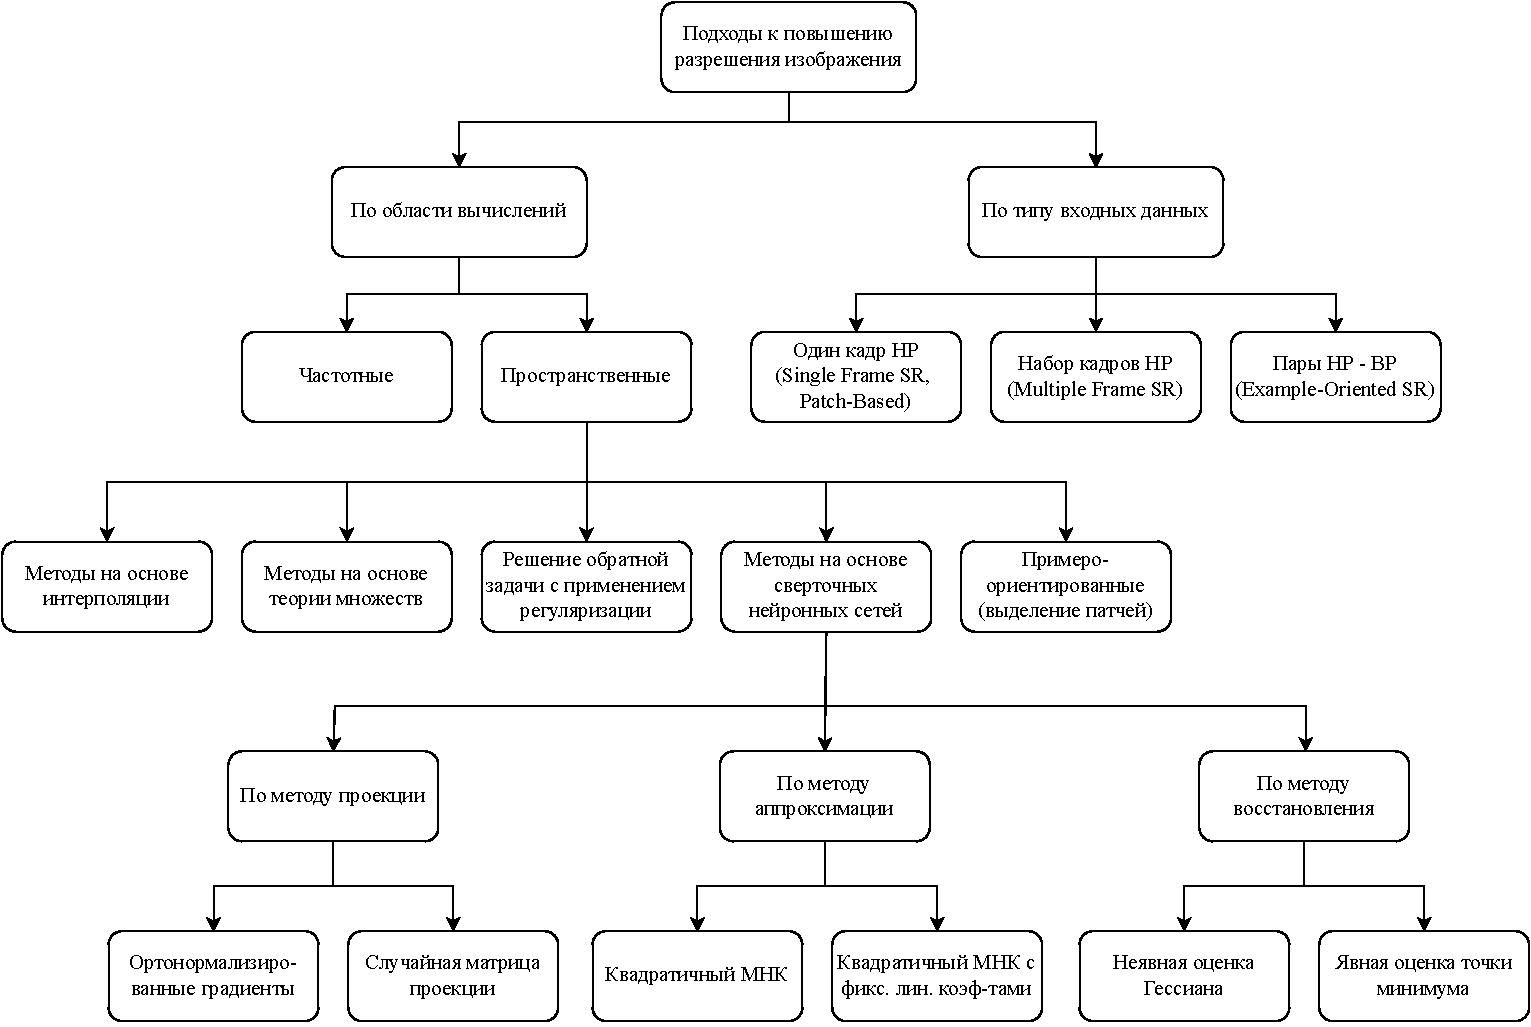
\includegraphics[scale=0.65]{assets/class}
	\caption{Классификация подходов повышения разрешения изображения}
	\label{class}
\end{figure}

\section{Сравнительный анализ рассмотренных методов суперрезолюции}

При сравнительном анализе методов повышения разрешения изображения были выделены следующие критерии: вычислительная сложность метода, качество обработки и необходимость пост~-- или предобработки.

В таблице 2.1 представлен сравнительный анализ рассмотренных методов.

\begin{sidewaystable}[h!]
    \centering
    \renewcommand{\arraystretch}{2}
    \caption{Сравнительный анализ рассмотренных методов}
    \begin{tabular}{|c|c|c|c|}
        \hline
        \multirow{2}{*}{Метод} & \multicolumn{3}{c|}{Критерий} \\
        \cline{2-4}
        & \specialcell{Вычислит. сложность} & \specialcell{Качество обработки} & \specialcell{Необходимость пост- или предобработки} \\
        \cline{2-4}
        \hline
        \specialcell{Частотные методы} & Низкая & Низкое & Нет \\
        \hline
        \specialcell{Интерполяционные методы} & Низкая & Очень низкое & Нет \\
        \hline
        \specialcell{Методы теории множеств} & Средняя & Низкое & Да \\
        \hline
        \specialcell{Регуляризация} & Средняя & Среднее & Нет \\
        \hline
        \specialcell{Выделение патчей} & Очень высокая & Высокое & Да \\
        \hline
        \specialcell{\textbf{СНС}} & \textbf{Высокая} & \textbf{Очень высокое} & \textbf{Да} \\
        \hline
    \end{tabular}
\end{sidewaystable}

%Достоинством метода является относительно низкая вычислительная сложность, что дает возможность получения результата в реальном времени. К недостаткам относится накопление и дальнешее распространение ошибки на этапе интерполирования значений.